In this chapter, we discuss the application of the methods from Chapter
~\ref{c:background} to the New York AirBnB dataset from Chapter
~\ref{c:methodology}.

\section{Training and Test Sets}
\label{sec:train_test_split}

The train-test split procedure is used to estimate machine learning algorithms'
performance when making predictions on data not used to train the model.  We
randomly split the dataset into 80\% and 20\% of listings for training and test
sets, respectively. The training set is used to fit the model, and the test
set is used to evaluate the fit machine learning model. The objective is to
estimate the machine learning model's performance on new data: data not used to
train the model.

The scikit-learn library provides an implementation of the train-test-split
procedure via the \texttt{train\_test\_split()} function.

\section{Findings}
\label{sec:findings}
A summary of of results is reported in Table ~\ref{tab:results}

\begin{table}[htpb]
  \centering
  \caption{Results}
  \label{tab:results}
  \begin{tabular}{lllll}
    \hline
    ML Algorithm & Training MSE & Test MSE & Training $R^2$ & Test $R^2$ \\
    \hline
    Linear Regresion & 0.1291 &  8.5E21 &  0.7019 & -1.9E22 \\
    Ridge Regression  & 0.1291 & 0.138 & 0.7019 &  0.6857 \\
    Lasso Regression & 0.1351 & 0.1441 & 0.688 & 0.6718 \\
    XGboost &  0.0798 & 0.1173 & 0.8157 &  0.7328 \\
  \end{tabular}
\end{table}


As expected in ~\ref{linear-regression} incorporating such a large number
of features (309) makes the linear regression model overfit the data. As
shown in Table ~\ref{tab:results}, while training MSE of the linear regression
model is quite good, the model performs poorly on the test set both in terms of
in terms of $MSE$ and $R^2$.

By performing k-fold cross-validation with ten folds, we can find the tuning
parameter's value that results in the smallest cross-validation error is 115.
The test's MSE is associated with this value of  is 0.138.  The result
represents a considerable improvement of ridge regression over the test MSE we
got using least square regression.


Using cross-validation , we find the optimized penalty value $\lambda$ for lasso
is 0.005.  The associated test MSE is 0.1441, which is slightly higher than the
test set MSE of the ridge regression.  Recall from that the advantage of using
lasso regression over ridge regression is that lasso performs feature selection.
Lasso picked 153 variables while eliminated the other 125 features.

%The figure ~\ref{fig:lasso-feature-importantance} shows the top 20 important
%features.

%\begin{figure}[H]\centering
    %\caption{Lasso Feature Importance}
    %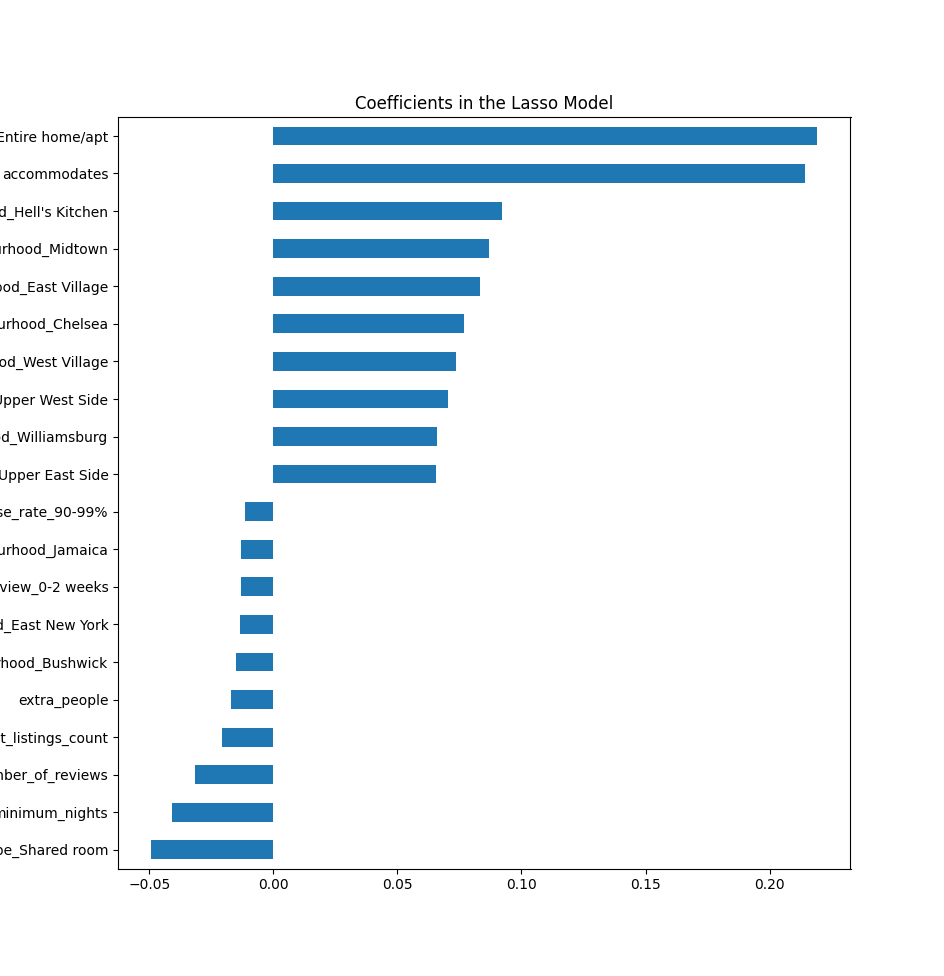
\includegraphics[width=\textwidth]{Figure_19.png}
    %\label{fig:lasso-feature-importantance}
%\end{figure}


%It is not surprising that the two most important positive features are whether
%the type of listing is the entire home and how many people the property
%accommodates. These are the main things a customer would use to search for
%properties in the first place.
%Features related to the location are in the top 10.  Being in  Hell's
%Kitchen, Midtown, East Village, Chelsea, West Village, Upper West Side,
%Williamsburg, Upper East Side, SoHo, Lower East Side neighbourhood is associated
%with an increase in the listing price.

As shown by the Table ~\ref{tab:results}, XGboost consistently outperforms these
competing approaches in both mean squared error and R-squared.  With this model,
the features explain approximately 73\% of the target variable's variance and
have smaller MSE than the other regression model.

\begin{table}[H]
  \centering
  \caption{XGBoost Top 20 Feature Weights}
  \label{tab:xgb-weights}
  \begin{tabular}{lr}
    \toprule
    {} &    weight \\
    \midrule
    room\_type\_Entire home/apt        &  0.336396 \\
    bathrooms                        &  0.032001 \\
    neighbourhood\_Midtown            &  0.025008 \\
    neighbourhood\_Hell's Kitchen     &  0.018545 \\
    neighbourhood\_East Village       &  0.015763 \\
    property\_type\_Other              &  0.015168 \\
    neighbourhood\_Bedford-Stuyvesant &  0.014314 \\
    neighbourhood\_West Village       &  0.014031 \\
    neighbourhood\_Chelsea            &  0.013612 \\
    neighbourhood\_Lower East Side    &  0.011874 \\
    neighbourhood\_Bushwick           &  0.011854 \\
    neighbourhood\_Upper West Side    &  0.011682 \\
    neighbourhood\_Washington Heights &  0.011659 \\
    neighbourhood\_SoHo               &  0.011582 \\
    room\_type\_Shared room            &  0.011304 \\
    neighbourhood\_Greenwich Village  &  0.010347 \\
    room\_type\_Hotel room             &  0.009697 \\
    neighbourhood\_Theater District   &  0.008575 \\
    neighbourhood\_Williamsburg       &  0.008490 \\
    neighbourhood\_Crown Heights      &  0.007979 \\
  \bottomrule
  \end{tabular}
\end{table}

Another important finding from \ref{tab:xgb-weights} was the role of location
features play in predicting price. In particular, location features located in
Manhattan and Brooklyn borough are in the top 20 important variables to predict
the price. This is consistent with what we observed in \ref{eda:neighbourhood}.
